\section{Decision Making}
\label{sec:decisionmaking}

The decision making is distributed in a master-slave topology, where all hall calls and cab calls are communicated with the master. The master updates a list of requests for each elevator which they want to serve. 

Which node who is the master is decided by the number of connections each node has and the duration each node has been alive. The master shall ping all slaves at regular intervals to communicate its presence and share system data. 

When an order is completed by an elevator it is removed from the local request list by that specific elevator and it is removed from the shared list of orders by the master. Only the latter should allow button lights to be deactivated.

All elevators send information about themselves to the master to allow for good decision-making

\section{Information}
\label{sec: information}
As there is a master-slave hierarchy, each elevator-computer should hold its own local data, as well as all the computers having a shared data that is syncronized as well. The data has been broken down as:

\begin{enumerate}
    \item Elevator-specific data:
    \begin{itemize}
        \item Current Floor: The elevator's current floor position.
        \item Destination Queue: A list of floors that the elevator is scheduled to stop at.
        Direction: The current direction of the elevator (up, down, or idle).
        \item Door Status: Whether the elevator doors are open, closed, or in the process of opening/closing.
        \item Occupancy Status: Information about the elevator's current load, which could be as simple as whether it's occupied or not, or more detailed occupancy data if sensors are available.
        \item Operational Status: Details about any faults or maintenance issues.
        \item Call Requests: Internal call requests from passengers inside the elevator (floors selected inside the elevator).
    \end{itemize}
    \item Shared System Data (synchronized between all computers):
    \begin{itemize}
        \item Floor Call Requests: Requests from each floor, including up and down buttons.
        \item Elevator Locations: The current floor of each elevator in the system.
        \item Elevator Directions: The current direction of travel for each elevator.
        \item System Time: To assist in uptime calculations and synchronization.
    \end{itemize}
    \item Master Computer-Specific Data:
    \begin{itemize}
        \item Global Call Assignment: Details of which elevator is responding to which call request.
        \item Elevator Status Overview: A summary of the status and availability of each elevator in the system.
        \item Uptime Records: Uptime for each computer to determine the master and slave hierarchy.
        \item System Logs: Logs of system activity for debugging and optimization purposes.
    \end{itemize}    
    \item Backup and Redundancy Data:
    \begin{itemize}
        \item Backup of Critical Data: Each computer should have a backup of critical operational data, so it can take over as master if necessary.
        \item Redundancy Plans: Procedures for handling the failure of one or more elevators or computers.
    \end{itemize}
    \item Communication Logs:
    \begin{itemize}
        \item Inter-Computer Communication: Records of communications between the computers for debugging and synchronization checks.
    \end{itemize}

    \item Performance Metrics:
    \begin{itemize}
        \item Operational Efficiency Data: Data on elevator usage patterns, response times, and efficiency, used for system optimization.
    \end{itemize}        
\end{enumerate}

\section{Communication protocol}
This project aims to use TCP as this way we will have a robust way of sharing and sending data. This way the computers will know whenever data has been sent successfully or not to determine if all computers are in sync. 

\section{Error Handling}
\label{sec:errorhandling}

If an elevator loses power, the hierarchy of elevators might be changed. If the master dies, the slave that has been alive the longest takes over as the new master.

If an elevator loses connection to all other elevators, but is still running, it will operate as one singular elevator keeping all hall and cab calls to itself.

If an elevator only loses connection to one other elevator, it might be de-ranked to slave. 



If a node is having some error and there is no active trip on this node, it should perform a reboot, so it might solve the issue.

\subsection{Network loss on node}
If a node loses connection to the network, it will no longer receive information from it's master, so after a certain time, the node restart the internet connection if it is in the idle state. This will be done by the computers pinging each other do determine whenever they have lost a connection to each other, and also pinging google or some other website to determine it it has lost connection or the other computers are faulty. If it doesn't recieve a response from both pings, then it knows that its not the master.

If the node that lost connection is the master, a new master will be appointed using the logic defined in \autoref{sec:decisionmaking}. 

\subsection{Packet Loss}
If a node doesn't confirm the packet received from the master, the TCP will send another packet until it's confirmed by the slaves. 

\subsection{}


\section{Programming Language}
We are going to use the programming language Go, since channels and go-routines are features that will work well for this type of project. The implementation of these are good for concurrency and deals with race condition. 


\section{Modules}

\subsection{Master module}
The master has some additional tasks, like decision making and delegating the different nodes to different assignments. in \autoref{fig:master_todo} the diagram shows how the master should proceed when a hallcall is given. 

\begin{figure}[H]
    \centering
    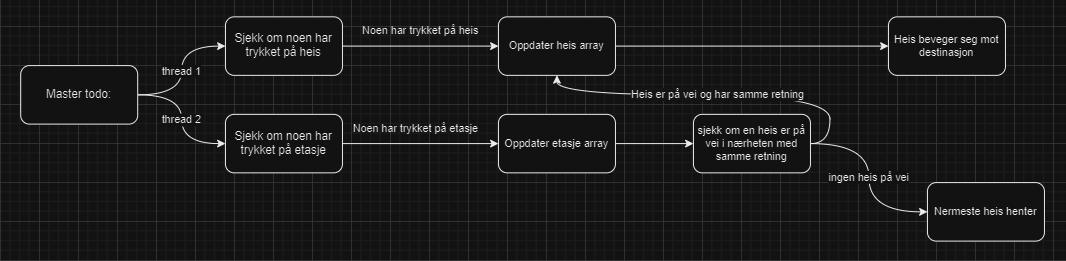
\includegraphics[width=\textwidth]{Latex/Images/Master_todo.png}
    \caption{How the master should when hallcall is received}
    \label{fig:master_todo}
\end{figure}

\subsection{Elevator Module}
Every node should work using this preliminary state diagram to show what states a node could be in. The transitions between states are assigned using local data on each node, where cabcalls are handled locally and hallcalls are handled by the master. 

\begin{figure}[H]
    \centering
    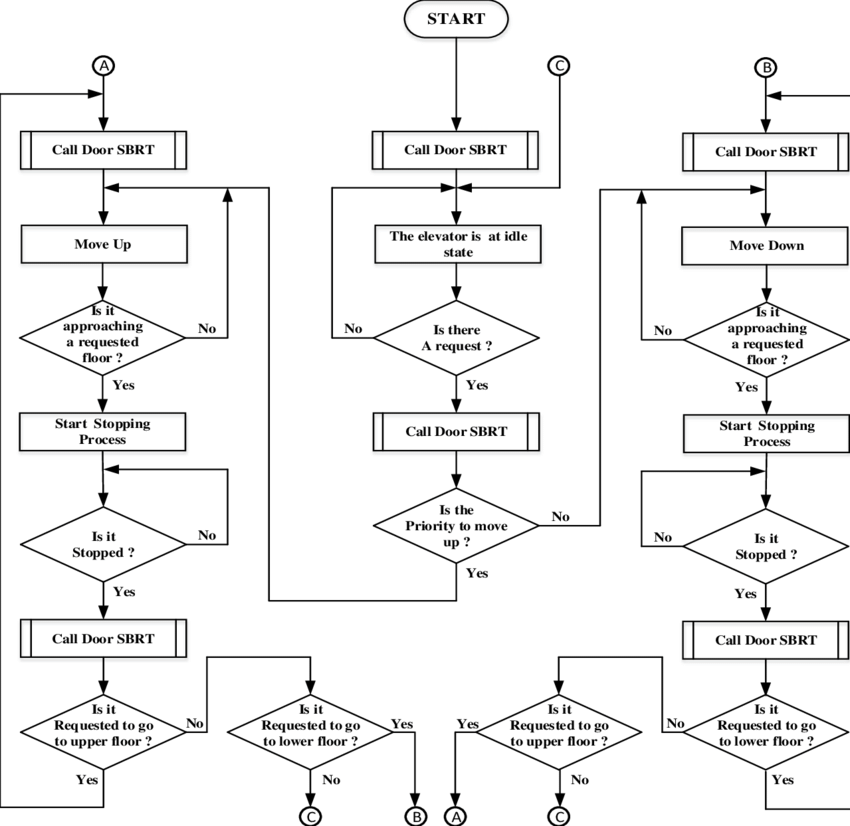
\includegraphics[width=\textwidth]{Latex/Images/418651894_696195342724008_4289962557826126166_n.png}
    \caption{A state diagram for each node}
    \label{fig:fsm_node}
\end{figure}

